\documentclass{lehramt-informatik-haupt}
\liLadePakete{cpm,mathe,gantt}

\begin{document}
\let\SZ=\liCpmSpaetesterI
\let\FZ=\liCpmFruehesterI

%%%%%%%%%%%%%%%%%%%%%%%%%%%%%%%%%%%%%%%%%%%%%%%%%%%%%%%%%%%%%%%%%%%%%%%%
% Theorie-Teil
%%%%%%%%%%%%%%%%%%%%%%%%%%%%%%%%%%%%%%%%%%%%%%%%%%%%%%%%%%%%%%%%%%%%%%%%

\chapter{CPM-Netzplantechnik}

\begin{liQuellen}
\item \cite{wiki:netzplantechnik}
\item \cite{wiki:methode-kritischer-pfad}
\end{liQuellen}

\noindent
Die Methode des kritischen Pfades wird auch
\memph{Tätigkeits-Pfeil-Darstellung} oder CPM-Netzplantechnik (von
englisch \memph{critical path method}, CPM)
genannt.\footcite{wiki:methode-kritischer-pfad}

\section{Netzplantechnik, DIN 69900-1}

„Netzplantechnik umfasst \memph{alle Verfahren} zur Analyse,
Beschreibung, Planung, Steuerung und Überwachung von \memph{Abläufen}
auf der \memph{Grundlage der Graphentheorie}, wobei Zeit, Kosten,
Einsatzmittel bzw. Ressourcen berücksichtigt werden können. Ein Netzplan
ist die graphische oder tabellarische Darstellung von Abläufen und deren
Abhängigkeiten“.
\footcite[Seite 14]{sosy:fs:3}

%-----------------------------------------------------------------------
%
%-----------------------------------------------------------------------

\section{Zentrale Begriffe}

Ein \memph{Vorgang} ist eine abgegrenzte Arbeitseinheit mit
\memph{Anfangs- und Endzeit} (vgl. Arbeitspaket im Projektmanagement).
Er besitzt eine \memph{Dauer}.
%
Unter Berücksichtigung der Dauer der einzelnen Vorgänge und unter
Berücksichtigung ihrer Abhängigkeiten wird ermittelt, wann die Vorgänge
stattfinden.
%
In CPM Netzen werden Vorgänge als \memph{Pfeile zwischen Ereignissen}
dargestellt.
\footcite[Seite 15]{sosy:fs:3}

\section{Zweck}

\begin{itemize}
\item Darstellen logischer Zusammenhänge
\item Zeitplan für alle Vorgänge entwickeln
\item Kritischer Pfad und Ressourcen-Engpässe identifizieren
\item Terminüberwachung, laufende Kontrolle
\end{itemize}

\section{Vier Teilaufgaben}

\begin{itemize}
\item Kapazitätsplanung
\item Kostenplanung
\item Strukturplanung
\item Zeitplanung / Zeitfenster
\end{itemize}
\footcite[Seite 22]{sosy:fs:3}

%-----------------------------------------------------------------------
%
%-----------------------------------------------------------------------

\section{Konstruktion eines Netzes}

Dem Vorgang $A_k$ wird ein Pfeil $e_k$ zugeordnet und mit dessen Dauer
bewertet.
%
$i_k$ und $j_k$ sind Anfangs- und Endereignis.
%
Die Anordnung erfolgt nach der Ende-Start-Beziehung.

\begin{center}
\begin{tikzpicture}
\liCpmEreignis[name=i]{$i_k$}{0}{0}
\liCpmEreignis[name=j]{$j_k$}{4}{0}
\liCpmVorgang{i}{j}{$e_k$}
\end{tikzpicture}
\end{center}

\begin{description}

\item[Regel 1:] Folgen die Vorgänge $A_3$ und $A_4$ unmittelbar $A_1$
und $A_2$ so gilt:
\footcite[Seite 24]{sosy:fs:3}

\begin{center}
\begin{tikzpicture}
\liCpmEreignis[name=1]{$i_1$}{0}{2}
\liCpmEreignis[name=2]{$i_2$}{0}{0}

\liCpmEreignis[name=m]{}{2}{1}

\liCpmEreignis[name=3]{$j_3$}{4}{2}
\liCpmEreignis[name=4]{$j_4$}{4}{0}

\liCpmVorgang{1}{m}{$e_1$}
\liCpmVorgang{2}{m}{$e_2$}
\liCpmVorgang{m}{3}{$e_3$}
\liCpmVorgang{m}{4}{$e_4$}
\end{tikzpicture}
\end{center}

\item[Regel 2:] Gibt es zwei Vorgänge (parallele Arbeitspakete) mit
demselben Anfangs- und Endereignis, so wird das Endereignis gesplittet
und ein Scheinvorgang eingeführt:
\footcite[Seite 25]{sosy:fs:3}

\begin{center}
\begin{tikzpicture}
\liCpmEreignis[name=1]{$i_1$}{0}{1}
\liCpmEreignis[name=2]{$j_2$}{4}{2}
\liCpmEreignis[name=3]{$j_3$}{4}{0}

\liCpmVorgang{1}{2}{$e_1$}
\liCpmVorgang{1}{3}{$e_2$}
\liCpmVorgang[schein]{2}{3}{$e_0$}
\end{tikzpicture}
\end{center}

\item[Regel 3:] Folgt der Vorgange $A_4$ unmittelbar $A_1$ und $A_2$ und
folgt $A_5$ unmittelbar $A_1$ , $A_2$ und $A_3$ so wird ein
Scheinvorgang eingeführt:
\footcite[Seite 26]{sosy:fs:3}
\end{description}

\begin{center}
\begin{tikzpicture}
\liCpmEreignis[name=1]{$i_1$}{0}{4}
\liCpmEreignis[name=2]{$i_2$}{0}{2}
\liCpmEreignis[name=3]{$i_3$}{0}{0}

\liCpmEreignis[name=4]{$j_4$}{4}{3}
\liCpmEreignis[name=5]{$j_5$}{4}{0}

\liCpmEreignis[name=m1]{}{2}{3}
\liCpmEreignis[name=m2]{}{2}{0}

\liCpmVorgang{1}{m1}{$e_1$}
\liCpmVorgang{2}{m1}{$e_2$}
\liCpmVorgang{3}{m2}{$e_3$}

\liCpmVorgang{m1}{4}{$e_4$}
\liCpmVorgang{m2}{5}{$e_5$}

\liCpmVorgang[schein]{m1}{m2}{$e_0$}
\end{tikzpicture}
\end{center}

\noindent
Es gibt nur eine Quelle (Projektstart) und eine Senke (Projektende).
Ggf. müssen Scheinvorgänge eingeführt werden, um dies zu erreichen.
%
Kann ein Vorgang $A_2$ bereits begonnen werden, wenn ein Teil des
Vorgangs $A_1$ erledigt ist, so wird $A_1$ gesplittet.\footcite[Seite
27]{sosy:fs:3}

\section{Beispiel\footcite[Seite 16 - 21]{sosy:fs:3}}

\begin{center}
\begin{tikzpicture}
\liCpmEreignis{1}{0}{2}
\liCpmEreignis{2}{1}{3.5}
\liCpmEreignis{3}{3}{2}
\liCpmEreignis{4}{2}{0.5}
\liCpmEreignis{5}{4}{3.5}
\liCpmEreignis{6}{5}{2}
\liCpmEreignis{7}{5}{0.5}
\liCpmEreignis{8}{7.5}{2}

\liCpmVorgang{1}{2}{5}
\liCpmVorgang{1}{3}{18}
\liCpmVorgang{1}{4}{7}
\liCpmVorgang{4}{7}{15}
\liCpmVorgang{7}{8}{6}
\liCpmVorgang{3}{6}{8}
\liCpmVorgang{3}{7}{1}
\liCpmVorgang{2}{5}{14}
\liCpmVorgang{5}{8}{11}
\liCpmVorgang{6}{8}{4}
\end{tikzpicture}
\end{center}

\begin{description}

%%
%
%%

\item[Vorwärtsterminierung:] $+$, bei Auswahl Maximum

\begin{description}
\item[\FZ] Frühester Zeitpunkt, zu dem Ereignis $i$ eintreten kann
\item[FAZ] = Frühester AnfangsZeitpunkt für Vorgang
\item[FEZ] = Frühester EndeZeitpunkt für Vorgang
\end{description}

\begin{tabular}{|l|l|l|}
i & Nebenrechnung & \FZ \\
1 &               & 0 \\
2 &               & 5 \\
3 &               & 18 \\
4 &               & 7 \\
5 &               & 19 \\
6 &               & 26 \\
7 & max(19,22)    & 22 \\
8 & max(30,30,28) & 30 \\
\end{tabular}

%%
%
%%

\item[Rückwärtsterminierung:] $-$, bei Auswahl Minimum

\begin{description}
\item[\SZ] Spätester Zeitpunkt, zu dem Ereignis $i$ eintreten kann
\item[SAZ] = Spätester AnfangsZeitpunkt für Vorgang
\item[SEZ] = Spätester EndeZeitpunkt für Vorgang
\end{description}

%%
%
%%

\item[Puffer:]

GP: gesamter Pufferzeit ($\text{GP} = \text{SZ} - \text{FZ}$)

%%
%
%%

\item[Kritische Pfade:]
Pfad(e) mit minimaler Pufferzeit, meist $0$

\end{description}

\begin{tabular}{|l|l|l|l|l|l|l|l|l|}
\hline
$i$           & 1 & 2 & 3  & 4 & 5  & 6  & 7  & 8  \\\hline\hline
\FZ & 0 & 5 & 18 & 7 & 19 & 26 & 22 & 30 \\\hline
\SZ & 0 & 5 & 18 & 9 & 19 & 26 & 24 & 30 \\\hline
GP            & 0 & 0 & 0  & 2 & 0  & 0  & 2  & 0  \\\hline
\end{tabular}

\bigskip

\bigskip

\begin{tabular}{|l|r|r|}
\hline
$i$ & Nebenrechnung & \SZ \\
\hline\hline
1 & \f$30 - \t{11}(5-8) - \t{14}(2-5) -\t{5}(1-2) = 0$ & \\
  & \f$30 - \t{4}(6-8) - \t{8}(3-6) - \t{18}(1-3) = 0$ & \\
  & \f$30 - \t{6}(7-8) - \t{15}(4-7) - \t{7}(1-4) = 2$ & \\
  & \f$\min(0,0,2)$ & 0 \\\hline

2 & \f$30 - \t{11}(5-8) - \t{14}(2-5) = 5$ & 5 \\\hline
3 & \f$30 - \t{4}(6-8) - \t{8}(3-6) = 18$  & \\
  & \f$30 - \t{6}(7-8) - \t{1}(3-7) = 23$  & \\
  & \f$\min(18,23)$                        & 18 \\\hline

4 & \f$30 - \t{6}(7-8) - \t{15}(4-7)$      & 9 \\\hline
5 & \f$30 - \t{11}(5-8)$                   & 19 \\\hline
6 & \f$30 - \t{4}(6-8)$                    & 26 \\\hline
7 & \f$30 - \t{6}(7-8)$                    & 24 \\\hline
8 & \f{}siehe $\text{FZ}_8$                & 30 \\\hline
\end{tabular}

\literatur

\end{document}
